\documentclass{standalone}
\usepackage{hsbcommon}
\makeatletter\AtBeginDocument{\@buildstepset{1,2,3,4,5}}\makeatother
\begin{document}
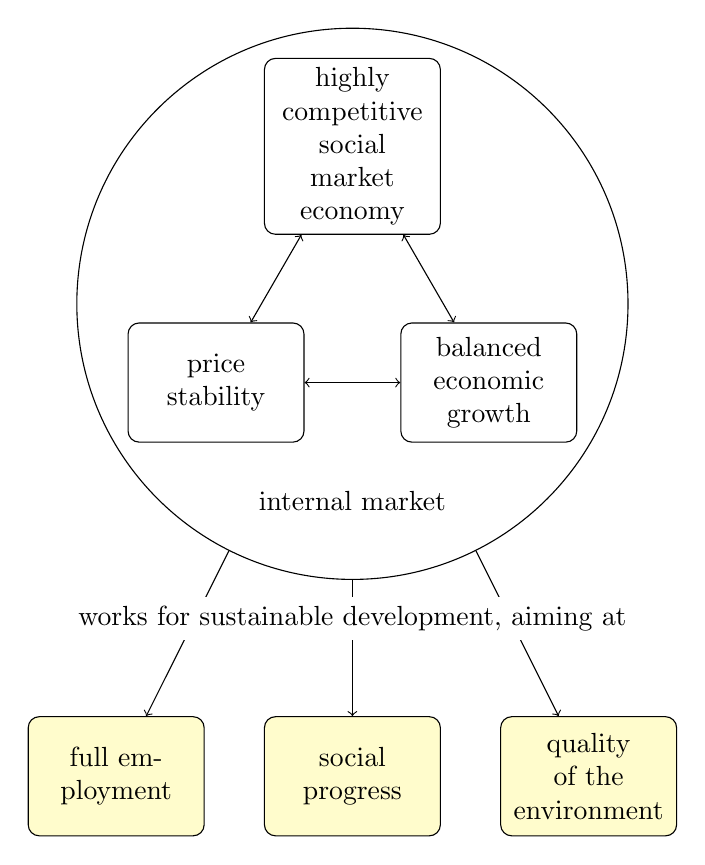
\begin{tikzpicture} 
    \tikzset{
        goal/.style={
            draw,
            text width=2cm,
            minimum height=10ex,
            align=center,
            rounded corners
        }
    }
    \foreach [count=\i] \myziel in 
    {%
    price stability,
    balanced economic growth,
    highly competitive social market economy%
    }
    {
        \node[goal] (N\i) at (120*\i+90:2) {\myziel};
    }
    \draw[<->] (N1) -- (N2);
    \draw[<->] (N2) -- (N3);
    \draw[<->] (N3) -- (N1);

    \node[draw,circle,minimum width=7cm] (O) at (0:0) {};
    \node  at (0,-2.5) {internal market};

    

        \foreach [count=\i] \myziel in 
            {%
            full employment,
            social progress,
            quality of the environment%
            }
            {
                \node[goal, fill=yellow!20] (M\i) at (3*\i-6,-6) {\myziel};
            }

    \draw[->] (O) -- (M1);
    \draw[->] (O) -- (M2);
    \draw[->] (O) -- (M3);

    \node[fill=white] at (0,-4) {works for sustainable development, aiming at};

    
\end{tikzpicture}
\end{document}
